\documentclass[11pt, a4paper]{article}

\usepackage{amsmath}
\usepackage{amssymb}

% fonts
\usepackage{xeCJK}
\setCJKmainfont[BoldFont=SimHei]{SimSun}
\setCJKfamilyfont{hei}{SimHei}
\setCJKfamilyfont{kai}{KaiTi}
\setCJKfamilyfont{fang}{FangSong}
\newcommand{\hei}{\CJKfamily{hei}}
\newcommand{\kai}{\CJKfamily{kai}}
\newcommand{\fang}{\CJKfamily{fang}}

% style
\usepackage[top=2.54cm, bottom=2.54cm, left=3.18cm, right=3.18cm]{geometry}
\linespread{1.5}
\usepackage{indentfirst}
\parindent 2em
\punctstyle{quanjiao}
\renewcommand{\today}{\number\year 年 \number\month 月 \number\day 日}

% figures and tables
\usepackage{graphicx}
\usepackage[font={bf, footnotesize}, textfont=md]{caption}
\makeatletter 
    \newcommand\fcaption{\def\@captype{figure}\caption}
    \newcommand\tcaption{\def\@captype{table}\caption}
\makeatother
\renewcommand\figurename{图}
\renewcommand\tablename{表}
\newcommand{\fref}[1]{\textbf{图\ref{#1}}}
\newcommand{\tref}[1]{\textbf{表\ref{#1}}}
\newcommand{\tabincell}[2]{\begin{tabular}{@{}#1@{}}#2\end{tabular}} % multiply lines in one grid

\usepackage{listings}
\lstset{basicstyle=\ttfamily}

\usepackage{clrscode}
\usepackage{url}

% start of document
\title{\hei 网格简化实验报告}
\author{\kai \quad 计35 \quad 朱俸民 \quad 2012011894}
\date{\kai \today}

\begin{document}

\maketitle

\section{综述}

实现基于边坍塌 (edge-collapse) 的网格简化 (mesh simplification) 方法。

\section{功能实现}

我们实现了以下功能:

\begin{itemize}
    \item 保持拓扑结构的简化;
    \item 支持两种收缩点的选择:(1) 中点;(2) 线性优化。
\end{itemize}

\section{效果分析}

\fref{s1}-\fref{s3}是对\texttt{Buddha.obj}模型采取不同简化比得到的结果(收缩点采用线性优化),可以看出其拓扑结构保持完整,但某些细节会随着简化比减小而减少。

\begin{center}
    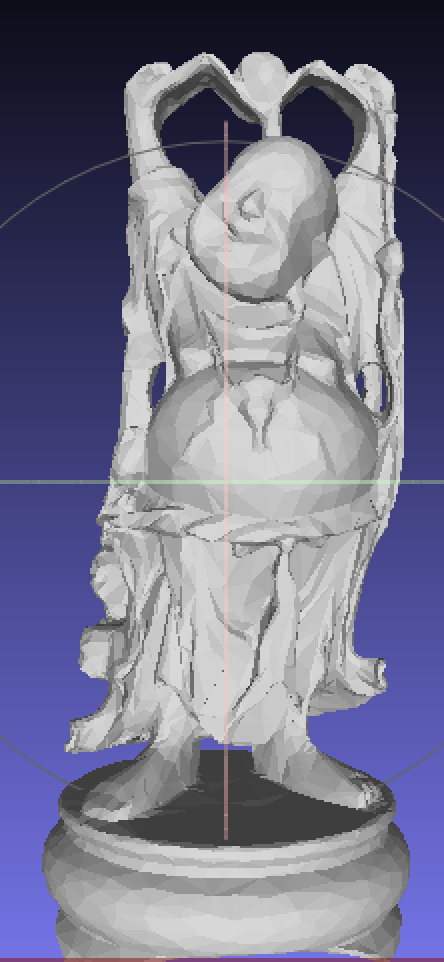
\includegraphics[width=4cm]{../output/buddha0.1.png}
    \fcaption{简化比0.1}\label{s1}
\end{center}

\begin{center}
    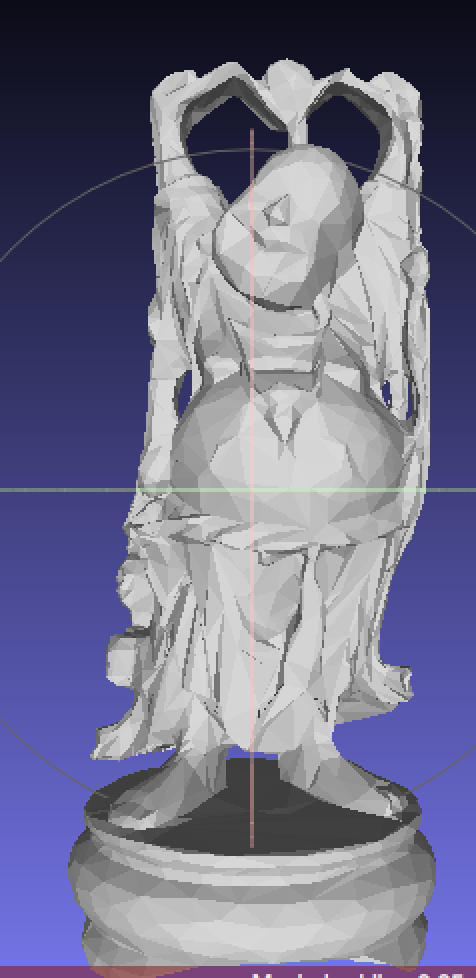
\includegraphics[width=4cm]{../output/buddha0.05.png}
    \fcaption{简化比0.05}\label{s2}
\end{center}

\begin{center}
    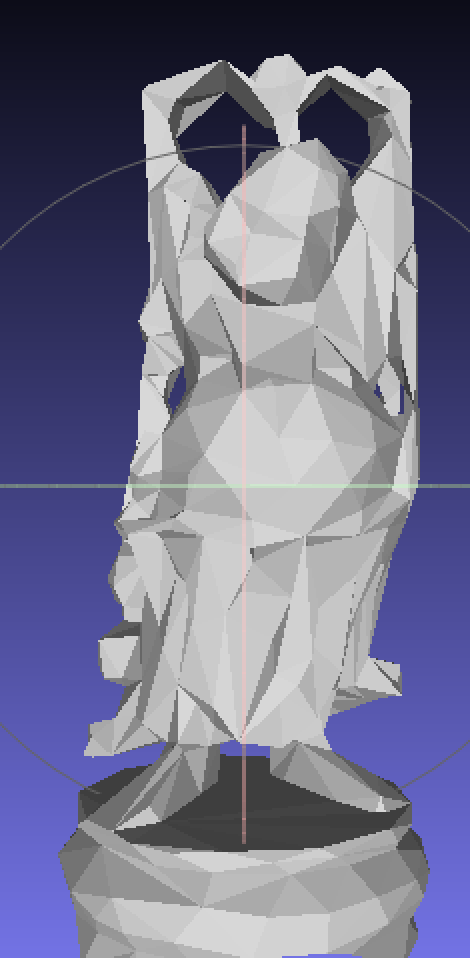
\includegraphics[width=4cm]{../output/buddha0.01.png}
    \fcaption{简化比0.01}\label{s3}
\end{center}

若采用中点作为收缩点,在简化比0.01时得到的结果如\fref{mid}所示。

\begin{center}
    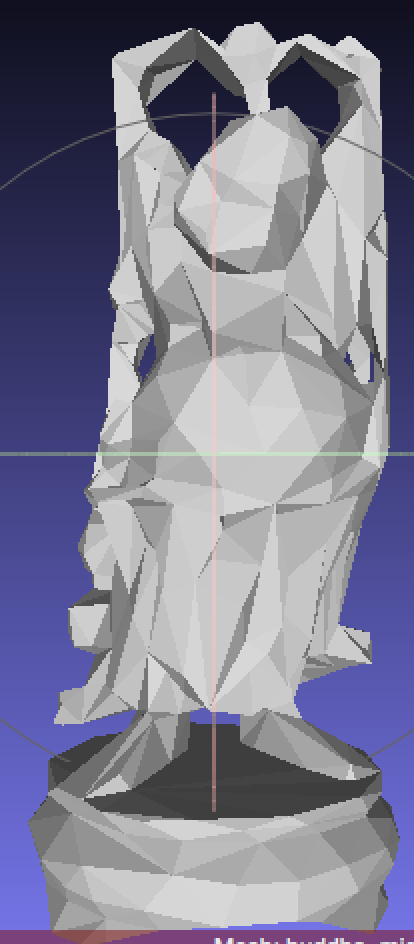
\includegraphics[width=4cm]{../output/buddham.png}
    \fcaption{利用中点作为收缩点,简化比0.01}\label{mid}
\end{center}

\section{用法}

请前往\url{https://github.com/paulzfm/MeshSimplification#mesh-simplification}查看。

\begin{thebibliography}{99}
    \bibitem{1} Prashant Chopra, Joerg Meyer. Topology Sensitive Volume Mesh Simplification with Planar Quadric Error Metrics. University of California, Irvine, Department of Electrical Engineering and Computer Science.
\end{thebibliography}

\end{document}